\documentclass[titlepage, a4paper, openbib, 10pt]{article}

%#####################################
%Usepackages en installingen
\usepackage[top=1in, bottom=1in, left=1in, right=1in]{geometry}
\usepackage[pdftex]{graphicx}
\usepackage{fancyhdr}
\usepackage{sectionbox}
\usepackage[dutch]{babel}
\usepackage{chngcntr}
\usepackage{cite}
\usepackage{url}
\usepackage{makeidx}
\usepackage{enumitem}
\usepackage{tocloft}
\usepackage{listliketab}	
\usepackage[table]{xcolor}
\usepackage{tabularx}
\usepackage{epsfig}
\usepackage{pdflscape}
\usepackage{pdfpages}
\usepackage{float}
\usepackage{multirow} 
\usepackage{rotating}
\usepackage[utf8]{inputenc}
\usepackage{listings}
\lstset{language=C,
basicstyle=\ttfamily\footnotesize,
frame=shadowbox,
mathescape=true,
showstringspaces=false,
showspaces=false,
breaklines=true}


%\usepackage{showframe} %tmp
%#####################################
%Nieuwe commando's
\newcommand{\HRule}{\rule{\linewidth}{1pt}}
\newcommand{\organisatie}{\uppercase{Hogeschool Rotterdam / CMI}}
\newcommand{\modulenaam}{Functioneel programmeren 1}
\newcommand{\modulecode}{\uppercase{TINFUN01}}
\newcommand{\stdPunten}{3 ects}
\renewcommand{\author}{Giuseppe Maggiore}

\definecolor{lichtGrijs}{RGB}{169,169,169}



%#####################################
%Index en styling
\setlength{\cftbeforesecskip}{10pt}
\setlength\parindent{0pt}
\makeindex
\graphicspath{{img}}
\counterwithin{figure}{subsection}
\pagestyle{fancy}
\setcounter{secnumdepth}{5}
\setcounter{tocdepth}{5}

%#####################################
%     Alles voor header/footer
\fancyhf[HL]{\nouppercase{\textit{\leftmark}}}
\setlength{\headheight}{36pt}
\lhead{\uppercase{\footnotesize Modulewijzer}}
\chead{\footnotesize \organisatie}
\rhead{
\includegraphics[width=0.09\textwidth]{img/logo}}

\lfoot{\scriptsize \modulenaam}
\cfoot{\scriptsize \today}
\rfoot{\small \thepage}

\renewcommand{\headrulewidth}{0.4pt}
\renewcommand{\footrulewidth}{0.4pt}
%#####################################

\begin{document}

%#####################################
%Titlepage
\begin{titlepage}
\thispagestyle{fancy}
\ 
\vspace{5cm}

\begin{center}

	
	\Large \textbf \organisatie
	
	\vspace{1.5cm}
	
	\HRule \\[0.4cm]
	
	\Huge \textbf \modulenaam
	
	\vspace{1.7cm}
	
	\Large \textbf  \modulecode
	
	\vspace{0.4cm}
	
	\HRule \\[1.5cm]
\end{center}
\vfill

% Author and supervisor
\begin{tabular}{l l}
	Aantal studieunten:  & \stdPunten\\
	Modulebeheerder: & \author\\
\end{tabular}

\end{titlepage}

%####### Contentpagina ########
%\renewcommand{\baselinestretch}{1.5}\normalsize
%\tableofcontents
%\newpage
%\listoffigures
%\newpage
%\listoftables
%\newpage

%########### Inhoud ###########

\shadowsectionbox
\section*{Modulebeschrijving}
\begin{tabularx}{\textwidth}{|>{\columncolor{lichtGrijs}} p{.26\textwidth}|X|}
	\hline
	\textbf{Modulenaam:} & \modulenaam\\
	\hline
	\textbf{Modulecode: }& \modulecode\\
	\hline
	\textbf{Aantal studiepunten \newline en studiebelastinguren:} & Deze module levert \stdPunten studiepunten op.
	\begin{itemize}
		\item 8 $\times$ 100 minuten hoorcollege
		\item 8 $\times$ 50 minuten practicum
		\item Het rest is zelfstudie
	\end{itemize} \\
	\hline
	\textbf{Toetsing:} & Schriftelijke toets en practicumopdrachten \\
	\hline
	\textbf{Werkvorm:} & Hoorcollege en practicum \\
	\hline
	\textbf{Vereiste voorkennis:}&Alle modules wiskunde en programmeren uit het eerste jaar en de eerste helft van het tweede jaar.\\
	\hline
	\textbf{Leermiddelen:}  &
		\begin{itemize}
			\item Boek: Types and Programming Languages, auteur: Benjamin Pierce
			\item Boek: Friendly F\# (Fun with game programming Book 1), auteurs: Giuseppe Maggiore, Giulia Costantini
			\item Text editors: Emacs, Notepad++, Visual Studio, Xamarin Studio, etc.
		\end{itemize} \\
	\hline
	\textbf{Draagt bij aan \newline competenties:} &
	\begin{center}
		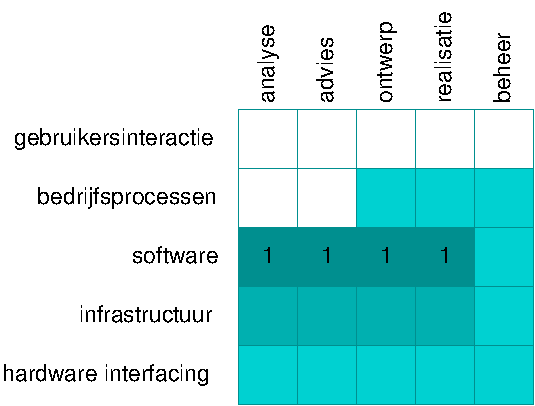
\includegraphics[width=7cm]{img/comptabel.pdf}
	\end{center}\\
	\hline
	\textbf{Leerdoelen:}&
	\begin{itemize}
		\item Het kunnen adviseren over en analyseren, ontwerpen en realiseren van een computerprogramma op niveau 1 (leerdoel A).
		\item Het kunnen ontwerpen, schrijven, compileren en uitvoeren van een correct werkend ML programma (leerdoel O).
		\item Het in correct Nederlands en met gebruikmaking van het juiste jargon kunnen communiceren over de programmeertaal (leerdoel C).
	\end{itemize} \\
	\hline
	\textbf{Inhoud:}&
	\begin{itemize}
		\item Programmeerparadigma's;
		\item Elementaire taalconstructies.
	\end{itemize}\\
	\hline
	\textbf{Modulebeheerder:} & \author\\
	\hline
	\textbf{Datum:} & \today \\
	\hline
\end{tabularx}
\newpage
\newpage
\section{Algemene omschrijving}
	\subsection{Inleiding}
		Functioneel programmeren is een in opkomst zijnde manier van programmeren die nogal wat verschillen vertoont met de klassiek imperatieve manier van programmeren zoals dit bekend is in programmeertalen als C, C++, Java e.v.a. \\ 

		Functionele talen zijn gebaseerd op de zogeheten \emph{$\lambda$ calculus}, waardoor deze talen fundamenteel anders werken dan de meeste programmeurs gewend zijn. Daar puur functionele talen geen side effects kennen en bovendien referential transparency gebruiken i.p.v. destructive update betekent dat programma's geschreven met functionele talen hebben hogere textit{encapsulation} van functies en data structuren, en vervolgens minder bugs en algemene fouten. Met het steeds populairder worden van deze platformen wordt ook het functioneel programmeren populairder. \\

		Verder is te zien dat met het steeds verder toenemen van het abstractieniveau, waarop computerprogramma' s functioneren de behoefte aan talen, waarin deze abstracties compact kunnen worden uitgedrukt, toeneemt. Functionele talen lijken hier tot nu toe de betere papieren voor te hebben.\\

	\subsection{Relatie met andere onderwijseenheden}
		Op deze module wordt voortgebouwd in de module TINFUN02. \\
	\subsection{Leermiddelen}
		Verplicht:
		\begin{itemize}
			\item Presentaties die gebruikt worden in de hoorcolleges (pdf): te vinden op N@tschool
			\item Opdrachten, waaraan gewerkt wordt tijdens het practicum (pdf): te vinden op N@tschool
		\end{itemize}
		Facultatief:
		\begin{itemize}
			\item Boek: Types and Programming Languages, auteur: Benjamin Pierce
			\item Boek: Friendly F\# (Fun with game programming Book 1), auteurs: Giuseppe Maggiore, Giulia Costantini
			\item Text editors: Emacs, Notepad++, Visual Studio, Xamarin Studio, etc.
		\end{itemize}
\newpage
\section{Programma}
	De volgende lijst zijn de onderwerpen van de cursus:
	\begin{enumerate}
		\item Inleiding, interpreter, eerste programma;
		\item Let, let-rec, basale flow-controle;
		\item Primitive types, tuples, type sommen, pattern-matching;
		\item Recursieve data-structuren, lijsten;
		\item Records;
		\item Hogere-orde-functies (HOF's);
	\end{enumerate}
\ \\


\newpage
\section{Toetsing en beoordeling}
	\subsection{Procedure}
		Deze module wordt getoetst middels een aantal practicumopdrachten. Deze opdrachten zijn te vinden op N@tschool.

		Voorwaarden en uitgangspunten:
		\begin{itemize}
			\item De practicumopdrachten bepalen het eindcijfer.
			\item De practicumopdrachten bestaan uit een game/simulatie voorbeeld die is niet compleet of foutieve; studenten moeten elke voorbeeld uitbreiden of corrigeren totdat het werkt volgens de opdracht beschrijving.
			\item De practicumopdrachten moeten documentatie bevatten.
		\end{itemize}
		\ \\
		
		Voor deze manier van toetsen is gekozen om de volgende redenen:
		\begin{itemize}
			\item Door de gegeven bronnen studenten moeten code lezen en begrijpen (leerdoel A).
			\item Door deze bronnen te corrigeren of invullen moeten studenten code schrijven (leerdoel O).
			\item Door documentatie schrijven moeten studenten communiceren over hun code (leerdoel C).
		\end{itemize}

		De cijfer van elke practicum opdracht is bepaald door:
		\begin{itemize}
			\item Correctheid van puur, functionele code (gebruik van \texttt{mutable} and \texttt{ref} is verboden) (60\%).
			\item Compleetheid en helderheid van documentatie (20\%).
			\item Gebruik van functionele patronen en idiomen zoals gezien in de lessen (20\%).
		\end{itemize}

	\subsection{Opdrachten}
	
		\paragraph{Opdracht 1 - let, expressies, definitie van functies}
			Studenten moeten twee functies definiëren om de positie en snelheid van een object te bewerken. De eindresultaat is dat het object door het scherm valt met zwaartekrachtversnelling.

            De signatures van de functies en waarden dat moeten geïmplementeerd worden zijn:
			\begin{lstlisting}
updatePosition (y:float) (vy:float) (dt:float) : float
updateVelocity (y:float) (vy:float) (dt:float) : float
			\end{lstlisting}


		\paragraph{Opdracht 2 - tupels, if's}
			Studenten moeten één enkele functie definiëren om de positie en snelheid van een object te bewerken. De functie retourneert een tupels met twee elementen: de nieuwe positie en de nieuwe snelheid van het object. Als het object de rand van het scherm raakt, dan moet hij opspringen.
			
            De signatures van de functies en waarden dat moeten geïmplementeerd worden zijn:
			\begin{lstlisting}
updateBall (y:float, vy:float) (dt:float) : float * float
			\end{lstlisting}


		\paragraph{Opdracht 3 - records}
			Studenten moeten twee records definiëren: \texttt{Vector2} en \texttt{MovingObject}. De \texttt{MovingObject} record bevat de positie en de snelheid van een object. Positie en snelheid zijn instanties van \texttt{Vector2}. Het object moet bewerkt worden zoals in \textit{Opdracht 2}, maar nu met 2D beweging.
			
            De signatures van de functies en waarden dat moeten geïmplementeerd worden zijn:
			\begin{lstlisting}
initialBall : Ball
updateBall (b:Ball) (dt:float) : Ball
			\end{lstlisting}


		\paragraph{Opdracht 4 - lijsten, pattern matching}
			Studenten moeten een recursieve functie definiëren om een lijst van \texttt{MovingObject}'s te bewerken. De functies van \textit{Opdracht 3} mogen gebruikt worden. Objecten die vallen buiten de randen van het scherm moeten van de lijst verwijdert worden.
			
            De signatures van de functies en waarden dat moeten geïmplementeerd worden zijn:
			\begin{lstlisting}
initialBalls : List<Ball>
rec updateBalls (balls:List<Ball>) (dt:float) : List<Ball>
rec removeOutOfBounds (balls:List<Ball>) : List<Ball>
			\end{lstlisting}


		\paragraph{Opdracht 5 - lijsten, hogere orde functies}
			Studenten moeten de functie van \textit{Opdracht 4} weer schrijven, maar door:
				\begin{itemize}
					\item eigen \texttt{map} en \texttt{filter} functies
					\item de standaard \texttt{map} en \texttt{filter} functies
				\end{itemize}

            De signatures van de functies en waarden dat moeten geïmplementeerd worden zijn:
			\begin{lstlisting}
rec map' (f:'a->'b) (l:List<'a>) : List<'b>
rec filter' (f:'a->bool) (l:List<'a>) : List<'a>
rec updateBalls' (balls:List<Ball>) (dt:float) : List<Ball>
rec removeOutOfBounds' (balls:List<Ball>) : List<Ball>

rec updateBalls''' (m:(Ball -> Ball) -> List<Ball> -> List<Ball>) (balls:List<Ball>) (dt:float) : List<Ball>
rec removeOutOfBounds''' (f:(Ball -> bool) -> List<Ball> -> List<Ball>) (balls:List<Ball>) : List<Ball>
			\end{lstlisting}


		\paragraph{Opdracht 6 - som types}
			Studenten moeten een 2D zoekboom (\textit{quadtree}) definiëren. Door dit zoekboom wordt het bepalen van collisies tussen kogels en asteroïden veel sneller ($O(N \log_4 N)$ in plaats van $O(N^2)$).

            De signatures van de functies en waarden dat moeten geïmplementeerd worden zijn:
			\begin{lstlisting}
type AsteroidQuadTree
rec treeToSeq (t:AsteroidQuadTree) : List<AsteroidQuadTree>
rec insert (a:Asteroid) (q:AsteroidQuadTree) : AsteroidQuadTree
rec existsColliding (p:Projectile) (q:AsteroidQuadTree) : bool
			\end{lstlisting}

			
		\paragraph{Opdracht 7 - abstracte datatypes}
			Studenten moeten een generieke collisie detectie functie. De functie bepaalt collisies tussen verschillende soorten van objecten. Om de vorm en positie van de objecten te bepalen gebruiken we een record van functies die specificeert hoe de generieke objecten uitgepakt moeten worden.
			
            De signatures van de functies en waarden dat moeten geïmplementeerd worden zijn:
			\begin{lstlisting}
let genericUpdate<'ship, 'asteroid, 'projectile>
  (s_ops:EntityOperations<'ship>)
  (a_ops:EntityOperations<'asteroid>)
  (p_ops:EntityOperations<'projectile>)
  (ship : 'ship, asteroids : List<'asteroid>, projectiles : List<'projectile>) (dt:float) 
  : 'ship * List<'asteroid> * List<'projectile>

let genericDraw<'ship, 'asteroid, 'projectile>
  (s_ops:EntityOperations<'ship>)
  (a_ops:EntityOperations<'asteroid>)
  (p_ops:EntityOperations<'projectile>)
  (spriteBatch:SpriteBatch)
  (ship : 'ship, asteroids : List<'asteroid>, projectiles : List<'projectile>) 
  : Unit


type Ship
shipOperations : EntityOperations<Ship>

type Asteroid
asteroidOperations : EntityOperations<Asteroid>

type Projectile
projectileOperations : EntityOperations<Projectile>
			\end{lstlisting}
			
			\textbf{Note: the above signatures are just a starting point.} The signatures, and the rest of the downloadable sources, may need to be adjusted in order to be made to work.


		\paragraph{Opdracht 8 - continuation passing style (CPS)}
			Studenten moeten twee kleine CPS functies schrijven: \texttt{faculteit} en \texttt{fibonacci}. Studenten moeten ook de zoekprocedure van \textit{Opdracht 6} weer schrijven met een variant van CPS die maakt het mogelijk om de procedure uit te voeren tot een aantal stappen (\textit{delayed/concurrent execution}).
			
			\textbf{Note: no signatures or code is provided.} As a very advanced assignment you are required to set up your own project from scratch.


	\subsection{Cijfers}
		De eerste vijf opdrachten zijn verplicht. Met deze opdrachten het is mogelijk om een zes cijfer te halen. Opdrachten zes en zeven zijn uitsluitend geldig als de eerste vijf opdrachten zijn correct. Met opdrachten zes en zeven de maximum cijfer mogelijk wordt een negen. De laatste opdracht is zeer moeilijk, en maakt het mogelijk om een tien te halen.
		
%##############################

\newpage
%\bibliographystyle{plain}
%\bibliography{references}
%\newpage
\section*{Bijlage 1: Toetsmatrijs}
	\begin{tabular}{|p{1cm}|p{4cm}|p{4cm}|p{4cm}|}
		\hline
		& Leerdoelen & Dublin descriptoren \\
		\hline
		1 & editor, compiler, source, binary, statements, declaratieve/imperatieve talen & 1,2,3,4 \\
		\hline
		2 & waarden: integer, float, double, boolean, char, String & 1,2,3,4 \\
		\hline
		3 & selectie: if, if-else, if-else-if, match-with & 1,2,3,4 \\
		\hline
		4 & recursie & 1,2,3,4 \\
		\hline
		5 & lijsten en recursieve data structuren & 1,2,3,4 \\
		\hline
		6 & HOF's en hun handeling & 1,2 \\
		\hline
		7 & lambda calculus & 1 \\
		\hline
	\end{tabular}
	
	\vspace{1cm}

	Dublin-descriptoren:
	\begin{enumerate}
		\item Kennis en inzicht
		\item Toepassen kennis en inzicht
		\item Oordeelsvorming
		\item Communicatie
	\end{enumerate}
%\newpage
%\section*{Bijlage 2: Voorbeeldtoets}

		Dit hoofdstuk bevat de beschrijving van de procedures om voor beoordeling in aanmerking te komen.\\
		Bijvoorbeeld voldoende aanwezigheid, 80\% van de opdrachten hebben ingeleverd, presentaties hebben verricht etc.\\

		Verder wordt zo gedetailleerd mogelijk beschreven hoe er tot een cijfer wordt gekomen en welke rollen er door docenten en ander betrokkenen hierbij vervuld worden. \\

		Geef een verantwoording van de toets; wat wordt getoetst, waarom is voor deze vorm gekozen.\\

		Vul een toetsmatrijs in voor de toets (zie bijlage).\\

		Beschrijf ook duidelijk de \textbf{herkansingsmogelijkheden}. \\

		Neem in geval van een schriftelijk tentamen een voorbeeldtoets op als bijlage.\\
		Geef daarbij per deelvraag het aantal te verdienen punten aan. \\

		Bij een schriftelijk rapport. Geef de beoordelingscriteria aan met daarbij de mogelijke score en de onderlinge weging. \\

		Toetsduur: \\

		Hoe en wanneer krijgt de student feedback?\\
%\newpage
%\section*{Bijlage 3: Studielast normering in ects}

		Dit hoofdstuk bevat de beschrijving van de procedures om voor beoordeling in aanmerking te komen.\\
		Bijvoorbeeld voldoende aanwezigheid, 80\% van de opdrachten hebben ingeleverd, presentaties hebben verricht etc.\\

		Verder wordt zo gedetailleerd mogelijk beschreven hoe er tot een cijfer wordt gekomen en welke rollen er door docenten en ander betrokkenen hierbij vervuld worden. \\

		Geef een verantwoording van de toets; wat wordt getoetst, waarom is voor deze vorm gekozen.\\

		Vul een toetsmatrijs in voor de toets (zie bijlage).\\

		Beschrijf ook duidelijk de \textbf{herkansingsmogelijkheden}. \\

		Neem in geval van een schriftelijk tentamen een voorbeeldtoets op als bijlage.\\
		Geef daarbij per deelvraag het aantal te verdienen punten aan. \\

		Bij een schriftelijk rapport. Geef de beoordelingscriteria aan met daarbij de mogelijke score en de onderlinge weging. \\

		Toetsduur: \\

		Hoe en wanneer krijgt de student feedback?\\
\printindex


\end{document}
